\documentclass{article}

\usepackage[hidelinks]{hyperref}
\usepackage[utf8]{inputenc}
\usepackage{float}
\usepackage{graphicx}
\graphicspath{ {assets/} }
\usepackage[backend=biber, style=authoryear-icomp]{biblatex}
\addbibresource{my.bib}

\newcommand{\comment}[1]{}

\usepackage[acronym]{glossaries}

\loadglsentries{glossary}
\makeglossaries

\begin{document}

\title{
	Software Requirement Specification \\
	for \\
	Bug-Tracker \\
	Version 1.0 approved
}
\author{Jesse Wood}
\maketitle
\newpage

\tableofcontents \label{contents}
\section{Introduction}
\subsection{Purpose}
\comment{
	Identify the product whose software requirements are specified in this document, including the revision or release number. Describe the scope of the product that is covered by the SRS. Particularly if this SRS describes only part of the system or a single subsytem.
	}
The product whose software requirements are specified in this document is a \Gls{bug}-tracker. \Gls{bug} tracking is a process of logging or monitoring bugs during software development \parencite{ibm20}. The software is a stand-alone system to be used as a bug-tracker while developing a project.
\subsection{Document Conventions}
\comment{
	Decribe any standards of typographical conventions that were followed when writing this \acrlong{srs}, such as fonts or highlighting that have special significance. For exmaple, state whether priorites for higher-level requirements are assumed to be inheritied by detailed requirements, or whether every requirement statement is to have its own priorities.
	}
This document follows the \acrshort{ieee} \acrshort{srs} convention \parencite{ieee20}. Fundamental requirements for this software will be explored in more detail than others.Each of the requirements will be listed in order of descending priority. All references can be found below in the \nameref{references}. Acronyms and technical terms can be found in the \nameref{glossary}. All of the UML diagrams used throughout the document were made using PlantUML \parencite{plantuml20}.
\subsection{Intended Audience and Reading Suggestions}
\comment{
Descibe the different types of reader that the document is inteded for, such as developers, project managers, marketing staff, users, testers, and documentation writers. Describe what the rest of the STS contains and how it is organised. Suggest a sequenc for reading the document, beginning with the overview sections and proceeding throught the sections that are most pertinent to each reader type.
}
The intended audience for this document is academics, developers and users. This document is set out sections defined in the table of contents \nameref{contents}, which explore different aspects of the systems requirements. Users of this software could find themselves only interested in a few sections, such as the \nameref{userDocumentation} or \nameref{systemFeatures}. Where as academics and developers may find the contents of the entire document to be relevant if they are looking into a similar software.
\subsection{Product Scope}\label{scope}
\comment{
Provide a short decription of the software being specified and its purpose, including relevant benefits, objectives and goals. Relate the software to corporate goals or business strategies. If a separate vision and scope document is available, refer to it rather than duplicating its contents here.
}
This software is designed to track bugs in projects. Bug-tracking is a useful way to develop large scale software and/or develop software in a team. A goal of this project will be to follow the \acrlong{mvc} design pattern \parencite{designpatterns97}. Using a design pattern will make the software reusable and easier to develop further in the future. Expanding on the \acrshort{mvc} model, maximising the modularity of this software will help make the project adaptable and promote further re-use in the future.
\newpage
\subsection{References}\label{references}
\comment{
If a seperate reader could access a copy of each reference, including title, author, version number, date, and source or location.
	}
Each of the following references are available in the form of an online pdf. Note that the availibility of website references may change subject to time.
\printbibliography
\newpage

\section{Overall Description}
\subsection{Product Perspective}
\comment{
Describe the context and origin of the product being specified in this \acrshort{srs}. For example, state whether this product is a follow-on member of a product family, a replacment for existing systems, or a new, self-contained product. If the \acrshort{srs} defines a component of a larger system, relate the requirments of the larger system to the functionality of this software and identift interfaces between the two. A simple diagram that shows the major components of the overall system, subsystem interconnections, and external interfaces can be helpful.
}
The development of this software originated out of necessity. One of the most crucial and time consuming tasks of any software development is the \gls{debugging} process. As software developers we plan to mimise the prevelance of bugs within our systems, however hard we may try, they will still perculate throughout our code bases. Bug-tracking is a process of managing bugs in a system into a priority hierarchy, such that each bug can be addressed with respect to the severity of its impact on the system. Another important part of a bug-tracker is the ability to change the status of a bug (e.g., when solved), this allows the workflow of a project to be monitored so that duplicate resources aren't assigned to fixing the same issue.

\subsection{Product Functions}
\comment{
	Summarize the major functions to the product must perform or must let the user perform. Details will be provided in Section 3, so only a high level summary (such as a bullet list) is needed here. Organize the functions to make them understandable to any ready of the SRS. A picture of the major groups of related requirements and how they relate, such as a top level data flow diagram or object class diagram, is often effective.
	}
\begin{figure}[h]
\caption{Class Diagram}
\centering
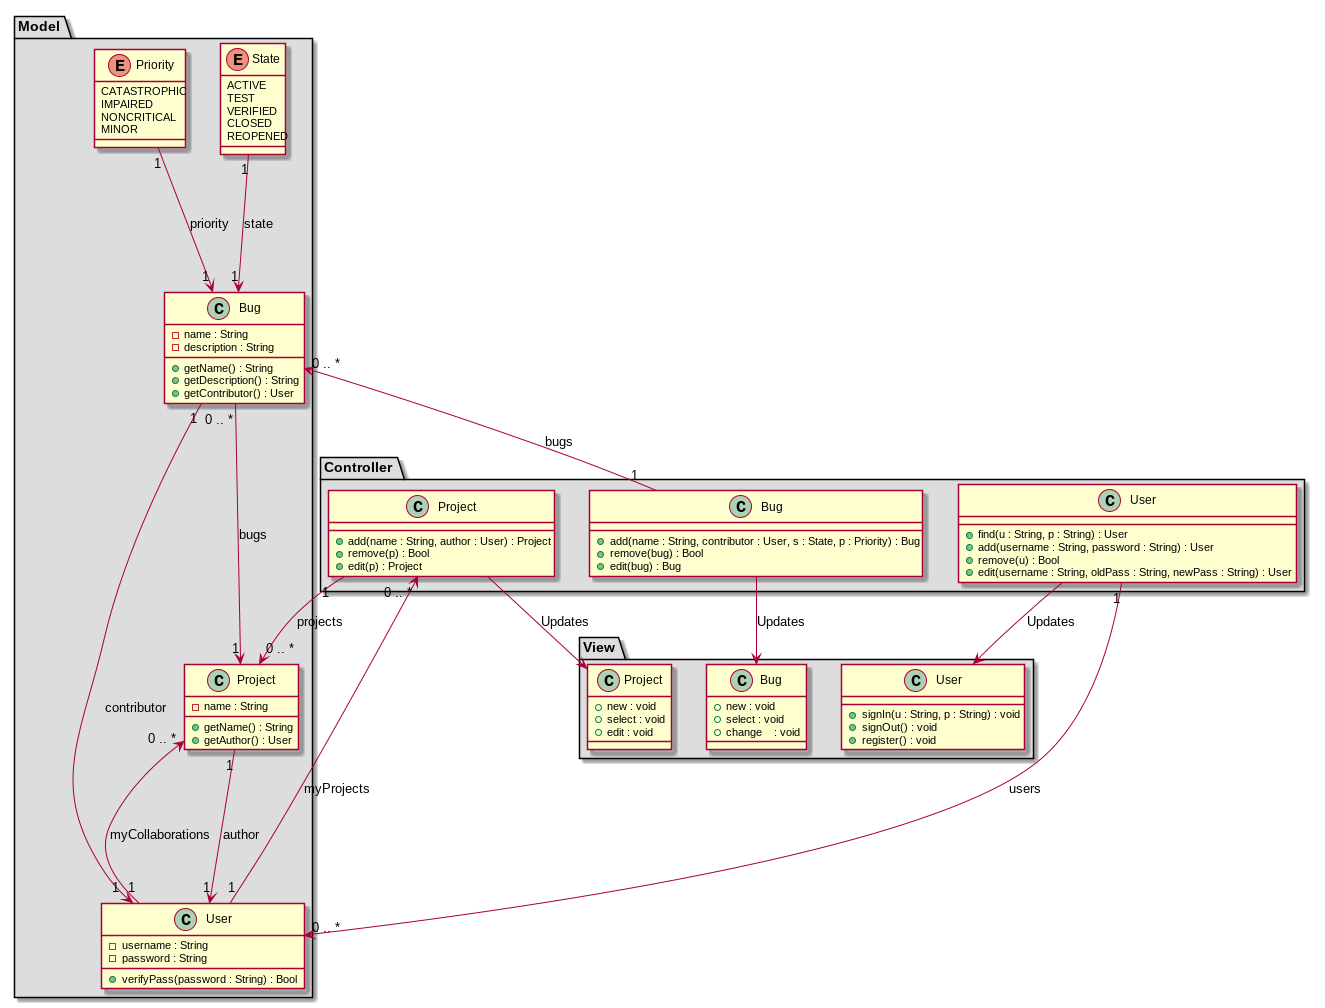
\includegraphics[width=\textwidth]{class-diagram.png}
\end{figure}
\subsection{User Classes and Characteristics}\label{userClass}
\comment{
Identify the various user classes that you anticipate will use this product. User classes may be differentiated based on the frequency of use, subset of product functions used, technical expertise, security or privelege levels, educational level, or experience. Describe the pertinent characteristics of each user class. Certain requirements may pertain only to certain user classes. Distinguish the most import user classes for this product from those who are less important to satisfy.
}
This software has three main user classes. The \emph{Author}, \emph{Colloborater} and \emph{Audience}. Each of these classes with have differently privelages related to a project.
\\ \\
An \emph{Author} has permission to delete and edit a project at will. They can also contribute bug reports and change the scope of a project from public to private or vice versa. An author is able to add/remove collaborators from a project, and remove any bug reports on their own projects.
\\ \\
A \emph{Collaborater} is an actor that has been granted permissions by the author. These privaleges allow the user to contribute bug reports to a project. However they cannot edit or delete the project itself.
\\ \\
The \emph{Audience} includes users that do not come under the aforementioned actors. They are able to view public projects. However they cannot contribute bug reports to these projects. Also they cannot view private projects.
\begin{figure}[h]
\caption{ Use Case Diagram}
\centering
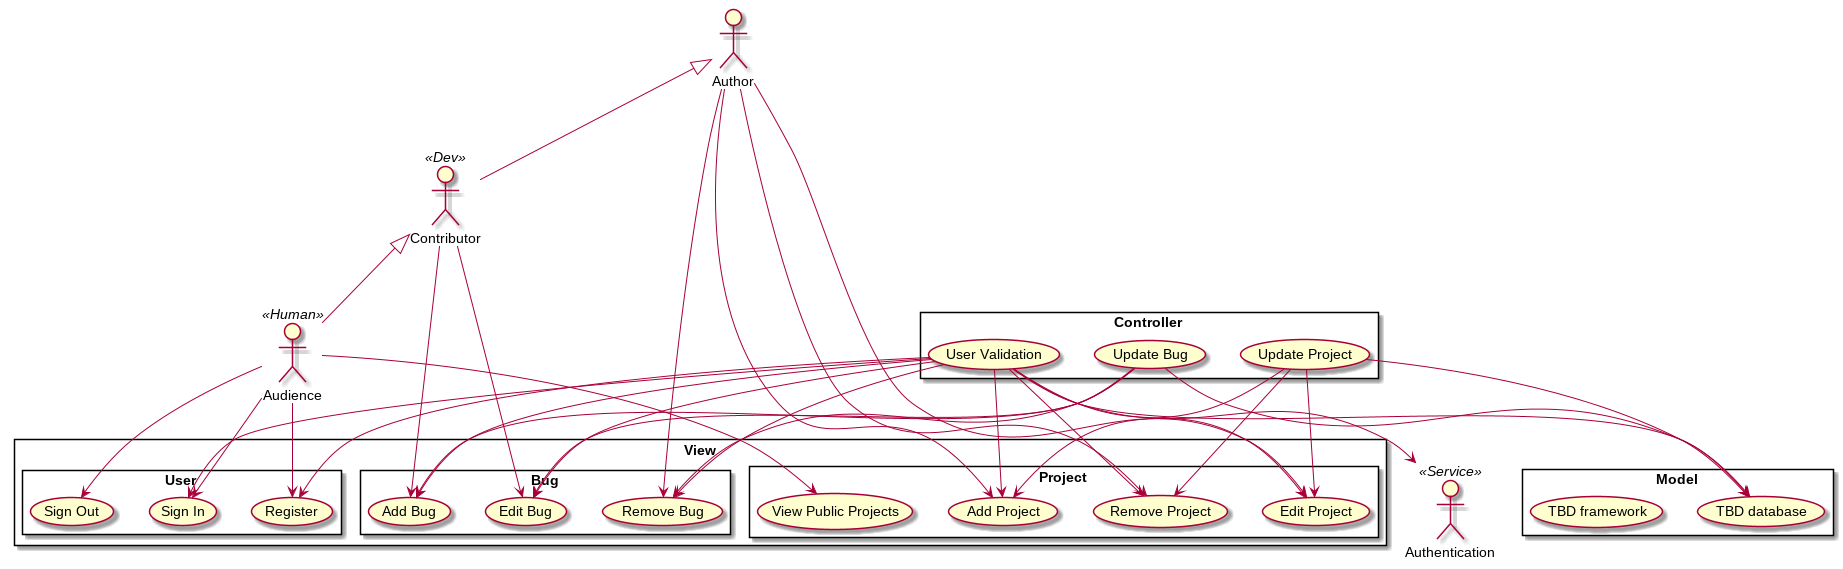
\includegraphics[width=\textwidth]{use-case-diagram.png}
\end{figure}
\subsection{Operating Environment}
\comment{
Describe the enviroment in which the software will operate, including the hardware platform, operating systems and versions, and any other software components or applications with which it must peacefully coexist.
	}
The software will be deployed in the form of a web app that relies on \acrshort{html}/\acrshort{css}/\acrshort{js} framework \acrfull{tbd}. These frameworks are constantly updated, so the software must be maintained over time, to ensure that future releases of the framework used do not introduce bugs. As long as the users' browswer supports the framework of the software, this system will be able to be run accross multiple operating systems. Therefore, only one version will have to be released. A more technical version of the software could be implemented for a terminal based environment for advanced use later if needed \acrshort{tbd}.
\subsection{Design and Implementation Constraints}\label{designConstraints}
\comment{
Descirbe any items or issues that will limit the options available to developers. These might include: corporate or regulatory policies; hardware limitations (timing requirements, memory requirements); interfaces to other applications; specific technologies, tools, and databases to be used, parallel operations; language requirements; communication protocols; security considerations; design conventions or programming standards (for example, if the customer's organization will be responsible for maintaining delivered software).
}
The \acrshort{tbd} \gls{database} system will be used to store the user informaiton. This introduces contraints to the storage capacity for user information. The amount of information stored cannot exceed the free-tier limit provided by the \acrshort{tbd} \gls{database} provider, or else the software will no longer be able to introduce new information.
\\ \\
Using a \gls{database} makes the software vulnerable to security exploits such as \acrshort{sql} Injection \parencite{sql20} and \acrshort{xss} \parencite{xss20}. The projects, bugs and user account informaiton will have to be stored in a \gls{database}. This is likely to hold sensitive information, especially the user information, therefore it is of paramount importance to ensure the software in secure against possible security exploits such as these.
\\ \\
The software will follow the design convention of \acrshort{mvc}. The \acrlong{mvc} is a very popular design pattern aimed at increasing flexibility and reuse \parencite{designpatterns97}. Developers intending to contribute to this project will have to follow the same design convention in any of their additions to the code base.
\\ \\
It would be expected that the software also follows the important principles of writing clean code \parencite{cleancode08}. Crafting software using these principles is pivotal to maintaing usable codebase.
\\ \\
Test driven development is a programming standard that is required during the development of this software. The increasingly popular DevOps approach it crucial in software development. Keep the test suit for this software up-to-date and all encompasing is of paramount importance to proving the functionality of the software.
\subsection{User Documentation}\label{userDocumentation}
\comment{
List the user documentation components (such as user manuals, on-line help, and tutorials) that will be delivered along with the software. Identify any known user documentation delivery formats or standards.
	}
The high-level components of the software will be documented in the source code. Following the documentation standards mentioned on the previous section \nameref{designConstraints}, the code-base of the software is well-documented for other developers.
\\ \\
\acrshort{tbd} Wiki eh. The code will have a Wiki available on the Github VCS for the software. This will explain the purpose for each of the individual components of the software at a high-level, with the in-line documentation providing further explanation when required.
\\ \\
\acrshort{tbd} Help section. On the web-page there is a help section. This includes FAQ with links to the Wiki for the relevant information a user and/or developer may require.
\subsection{Assumptions and Dependencies}
\comment{
List any assumed factors (as opposed to known facts) that could affect the requirements stated in the SRS. These could include third-party or commercial components that you plan to use, issues around the development environment, or constraints. The project could be affected if these assumptions are incorrect, are not shared, or change. Also identify any dependencies the project has on external factors, such as software components that you intent to reuse from another project, unless they are already documented elsewhere (for example, in the vision and scope document or the project plan)
	}
Javascript frameworks,
\\ \\
Vim is the text editor used to develop the software. Vim is a free and open source software. With the needed technical expertise, anyone can continux to develop this software, with no commerical software needed.
\\ \\
The project will be released under an MIT license. Therefore the reuse of the code and further development will follow the guidelines stipulated by this license \parencite{mit20}. It is assumed that developers and users of this software will adhere to the rules of the license it was released under.
\\ \\
Git is the Version Control System used to document the development of the project. It is assumed that any further development will follow git ettiquette. Improvements and re-works to the software can be forked of the master branch. Given the license, previously mentioned, further development of this software from other developers is welcome and encouraged.
\newpage

\section{External Interface Requirements}
\subsection{User Interfaces}
\comment{
	Describe the logical characteristics of each interface between the software product and users. This may include smaple screen images, any GUI standards or product family style guides that are to be followed, screen layout contraints, standard buttons and functions (e.g., help) that will appear on every screen, keyboard shortcuts, error message display standards, and so on. Define the software components for which a user interface is needed. Details of the user interface should be documented in a seperate user interface specification.
	}
The user interfaces for this software will be designed to work in a browser. The web app intefaces will be designed with mobile use considered. Therefore all of the following interfaces will also have cross-compbatibility with browsers on mobile devices. The user interface will be designed with usability being the primary focus. It will implement some common UI design conventions discussed in literature \parencite{aboutface14}
\\ \\
\begin{figure}[H]\label{sign-in}
\caption{Sign In}
\centering
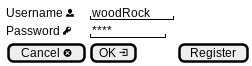
\includegraphics[width=0.5\textwidth]{sign-in.png}
\end{figure}
\begin{figure}[H]\label{register}
\caption{Register}
\centering 
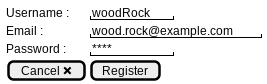
\includegraphics[width=0.5\textwidth]{register.png}
\end{figure}
The sign in screen is the first interface the user will see. This will allow the user to log in to their account. Google verification will be provided should a user not want to create their own account (\nameref{sign-in}).
\\ \\
\begin{figure}[H]\label{project}
\caption{Add a Project}
\centering
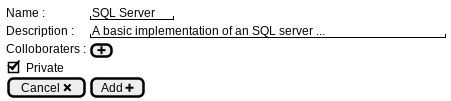
\includegraphics[width=0.5\textwidth]{project.png}
\end{figure}
\begin{figure}[H]\label{projects}
\caption{Projects Menu}
\centering
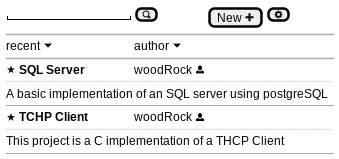
\includegraphics[width=0.75\textwidth]{projects.png}
\end{figure}
Another interface is the project menu. This allows the user to navigate to a particular project. With the possibility to create a new project, or find an existing one (\nameref{projects},\nameref{project}).
\\ \\
\begin{figure}[H]\label{bug}
\caption{Add a Bug}
\centering
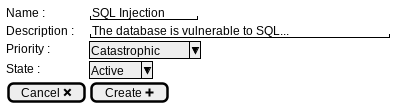
\includegraphics[width=0.5\textwidth]{bug.png}
\end{figure}
\begin{figure}[H]\label{bugs}
\caption{Project Menu}
\centering

\includegraphics[width=0.75\textwidth]{bugs.png}
\end{figure}
Each project has its own dashboard. On this interface a user can add/change the status of bugs. View the history of a project. Search for a bug within a project (\nameref{bugs}, \nameref{bug}).
\\ \\
Their will be a settings interface for the authors of projects. Given the correct log in credentials a user will be able to edit information about a project. Such as whether it is public or private, its name, remove a project ... etc.
\subsection{Hardware Interfaces}
\comment{i
Describe the logical and physical characteristics of each interface between the software product and the hardware components of the system. This may include the supported device types, the communication protocols to be used.
	}
The software supports any device that supports a \acrshort{tbd} browsers. It can run on Desktop, Laptop and Mobile devices so long as they support the \acrshort{tbd} framework.
\subsection{Software Interfaces}
\comment{
Describe the connections between this product and other specific software components (name and version) including databases, operating systems, tools, libraries, and integrated commercial components. Identify the data items or messages coming into the system and going out and describe the purpose of each. Describe the services needed and the nature of communications. Refer to documents that describe detailed application programmin interface protocols. Identify data that will be shared across software components. If the data sharing mechanisim must be implemented in a specific way (for example, use of a global data area in a multitasking operating system), specify this as an implementation constraint.
}
\acrshort{tbd}
The software requires a connection to an external \gls{database}. This stores all the information regarding the projects and their bugs. Using this software interface requires the use of queries as well as read and write access to the \gls{database}. The \gls{database} is able to concurrently accessed by multiple users. Using a robust \acrshort{dbms} ensures that this \gls{database} can be implemented.
\\ \\
Another software interface used is the \acrshort{tbd} framework. Libraries from this framework are used to implement the \acrshort{gui} and query/read/write to the \gls{database}. The software is implemented in a way such that all communication between the \gls{database} and framework uses an interface. This allows the code to be refactored easily should the choice of \gls{database} change in the future. Using the \acrshort{mvc} helps, such that the interactions with the \gls{database} can be compartmentalized into the model component.
\subsection{Communication Interfaces}
\comment{
	Describe the requirements associated with any communication functions required by this product, including e-mail, web-browswer, network server communication protocols, electronic forms, and so on. Define any pertinant message formatting. Identify any communication standards that will be used, such as FTP or HTTP. Specify any communication security or encryption issues, data transfer rates, and synchronization mechanisms.
}
The communication interface of email \acrshort{tbd} is used to allow notificaitons for projects. This includes letting the user know when new bugs are contributed or if the status of a bug changes. The user can edit the thresholds for certain notifications in the settings \acrshort{gui}.

\newpage
\section{System Features}\label{systemFeatures}
\comment{
E.g.

Description and Priority:
<Provide a short description of the feature and indicate whether it is of High, Medium or Low Priority. You could also include specific priority component ratings, such as benefit, penalty, cost, and risk (each rated on a relative scale from low of 1 to high of 9)>

Stimulus/Response Sequences:
<List the sequences of user actions and system responses that stimulate behaviour defined for this feature. These will correspond to the dialog elements associated with use cases.>

Functional Requirments:
< Itemize the detailed functional requirements associated with this feature. These are the software capabilites that must be present in order for the user to carry out the services provided by the feature, or to execute the use case. Include how the product should respond to anticipated error conditions or invalid inputs. Requirements should be concise, complete, unambigious, verifiable, and necessary. Use \acrshort{tbd} as a placeholder to indicate when necessary information is not yet available.>

<Each requirement should be uniquely identfied with a sequence number or a meaningful tab of some kind.>
	}
\subsection{Bugs}
A bug represents a software error. It is a brief description of a problem accompanied with a state and a priority.
\\ \\
Stimulus/Response Sequences
\begin{itemize}
\item create bug with a priority and state
\item change the state of a bug
\item record the bug contributor, time, etc ...
\end{itemize}
Functional Requirements:
\begin{itemize}
\item Each bug has one state and priority
\item Each bug is unique
\item Bugs store information about state changes
\item Bugs have a contributor
\end{itemize}
States for software bugs include:
\begin{itemize}
\item Active
\item Test
\item Verified
\item Closed
\item Reopened
\end{itemize}
Priorities for software bugs include:
\begin{itemize}
\item Catastrophic
\item Impaired Functionality
\item Failure of non-critical systems
\item Very Minor
\end{itemize}
\parencite{ibm20}

\subsection{Project}
A project represents a code base that a user intends to monitor bugs on. These can be added/removed/edited from/on the \gls{database}.
\\ \\
Stimulus/Response Sequences:
\begin{itemize}
\item create project
\item add/remove collaborators
\item add bugs to the project
\item View History of bugs
\item View Project information (collaboraters/author/date initiated)
\end{itemize}
Functional Requirements:
\begin{itemize}
\item Collaboraters/Author can edit project
\item Author can add/remove collaboraters to project
\item Author can edit details of the project
\item Bugs can be added/removed from a project
\end{itemize}

\subsection{Log-in}
This feature allows the user to log in and access their projects. This has Google authentication and also the ability for a user to register their own account, and sign in. This feature requires \gls{encryption}, such that the users sensitive information such as emails and passwords are not leaked.
\\ \\
Stimulus/Response Sequences
\begin{itemize}
\item A user can enter a username and password
\item Google Authentication
\item Register an account
\item A user can log in
\end{itemize}
Functional Requirements:
\begin{itemize}
\item No duplicate accounts
\item Strong passwords
\item store the account information securely
\item Account is linked to its own and collobaration projects
\end{itemize}
\newpage

\section{Other Nonfunctional Requirements}
\subsection{Performance Requirements}
\comment{
If there are performance requirements for the product under various circumstances, stat them here and explain their rationale, to help developers understand the intent and make suitable design choices. Specift the timing relationships for real time systems. Make such requirements as specific as possible. You may need to state performance requirements for individual functional requirements or features.
}
The \gls{database} must be able to handle \gls{con}. Since there will be multiple users attempting to access the information at the same time. Modern \acrshort{rdbms} like \gls{mysql} or \gls{postgresql} handle this. The rationale behind this is to allow multiple users to access the software at once. These users need to have the same results if performing the same actions.
\subsection{Safety Requirements}
\comment{
Specify those requirements that are concerned with possible loss, damage, or harm that could result from use of the product. Define any safeguards or actions that must be taken, as well as actions that must be prevented. Refer to any external policies or regulations that state safety issues that affect the product's design or use. Define any safety certifications that must be satisfied.
	}
Secure log in authentication is a safety requirement for this software. The software will have to meet the safety certifications Google requires to include Google Authentication. This requires the software to meet \gls{totp} algorithm specifications \parencite{totp11}. This can be implemented using \acrfull{js} frameworks. It is a requirement for this software. Users find software with Google Authentication more trustworthy and reputable.
\subsection{Security Requirements}
\comment{
Specify any requirements regarding security or privacy issues surrounding use of the product or protection of the data used or created by the product. Define any user identity authentication requirements. Refer to any external policies or regulations containing security issues that affect the product. Define any security or privacy certifications that must be satisfied.
	}
End to end data \gls{encryption} is requried for private projects for users. If a user sets a projects scope to private, it means for whatever reason they do not wish to make the contents of this project publicly available. It is in the best interest for developing this software that all the information regarding private projects remains encrypted. It will require a \gls{key} only available to the author of the project to decrypt the projects contents. This means should the private projects on the database leak, they will still remain encrypted in a non-human readible format.
\\ \\
\Gls{encryption} of user log-in information. It is important that the users' sensitive information, such as their passwords are stored on the database in an encrpted from. The authentication service can perform a \Gls{hash} Function \parencite{hash20}. This ensures that the password does not have to stored as a \gls{string} on the \gls{database}. Instead it can be stored as a \gls{hash}. Should the sensitive user information on the \gls{database} be released, the passwords will still remain encrypted.
\\ \\
\Gls{database} must be secure from \acrshort{sql} Injection and \acrshort{xss}. To prevent database leaks from even happening in the first place the program is required to be secure. For example, to prevent \acrshort{sql} injection any user input that interacts with the \gls{database} must be sanatized. This involves checking for hidden \acrshort{sql} code within user input, and sanatizing the input, before allowing it to be entered into the \gls{database}.
\\ \\
\subsection{Software Quality Attributes}
\comment{
Specify any additional quality characteristics for the product that will be omportant to either the customer or the developer. Some to consider are adaptability, availability, correctness, flexibility, interoperability, maintaintability, portability, reliability, reusability, robustness, testability, and usability. Write these to be specific, quantative and verifiable where possible. At least, clarify the relative preferences for various attributes, such as ease of use over ease of learning.dd
	}
The software demonstrates \gls{mod} through the use of the \acrshort{mvc} design pattern \parencite{designpatterns97}. This design pattern is an excellent example of \gls{mod} in a code base. It uses abstraction to seperate the software into three distincts modules which. The \acrfull{mvc} modules make future development of this software easier, even for new developers. So long as they are familiar with this common design pattern.
\\ \\
\Gls{test} is perhaps one of the most important aspects of developing reliable software. Through the use of \acrshort{tdd}, this software creates its own test suite during development. This test suite helps to demonstrate the functionality of the software. It make integration testing new features for un-intended side effects a piece of cake, since the test suite is already written. Using \acrshort{tdd} is one of the most effective ways to demonstrate that the software meets its own requirements.
\\ \\
\Gls{main} is a quality attribute that software inherits through \gls{mod} and \gls{test}. Focussing on \gls{mod} by using \gls{mvc} means that each module has low coupling. Using \gls{tdd} the test is written first, then the code to pass it. This means that extra functionality or dead code will not be prevelent in the code base. This in combination with the \gls{mod} will ensure high cohesion.
\subsection{Business Rules}
\comment{
List any principles about the product, such as which individuals or roles can perform which functions under specific circumstances. These are not functional requirments in themselves, but they may imply certain functional to enforce the rules.
	}
The individuals who can perform specific functions is explained in detial in this previous section, \nameref{userClass}. To reiterate the business rules for this software the reasoning behind this will be explained.
\\ \\
An \emph{Author} can Delete and Rename Projects and Bugs. This rule applies only to the projects they have created. This privelage is extended to the user such that they can manage their own projects. Colloboraters do not have these permissions because an author is the only actor that should be able to decide whether or not a project is needed.
\\ \\
\emph{Authors} and \emph{Collaborators} can see, add bugs, change status for private projects. Some projects may have more than one developer. The author is able to add one or more collobaraters to their own project. This allows a team to track bugs for a project. This functionality is not extended to the audience, this is because an author may not welcome the input of random contributors.
\\ \\
Lastly, the \emph{Audience} cant edit or post bugs without relevant permissions. They still have the ability to view the history of public projects. This adds a community aspect to the software. Users can see if other contributors have solved the same or similar bugs to what they are currently experiencing.
\newpage

\section{Other Requirements}
\comment{
	Define any other requirements not covered elsewhere in the \acrshort{srs}. This might include database requirements, internationalization requirments, legal requirments, reuse objectives for the projects, and so on. Add any new sections that are pertinent to the project.
	}
\subsection{Glossary}\label{glossary}
\comment{
Define all the terms necessary to properly interpret the \acrshort{srs}, including acronyms and abbreviations. You may wish to build a seperate gglossary that spans multiple projects or the entire organization, and just include terms specific to a single project in each \acrshort{srs}.
	}
\printglossary[type=\acronymtype]

\printglossary

\subsection{Analysis Models}
\comment{
Optionally, include any pertinent analysis models, such as data flow diagrams, class diagrams, state-transition diagrams, or entity-relationship diagrams.
	}
\begin{figure}[h]
\caption{ Sign In Sequence Diagram }
\centering
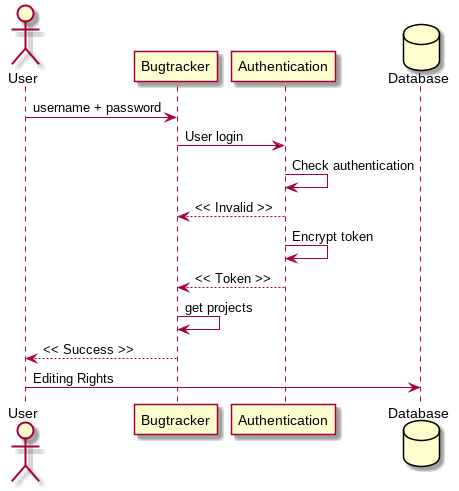
\includegraphics[width=\textwidth]{sequence-diagram.png}
\end{figure}
\subsection{To Be Determined List}
\comment{
Collect a numbered list of the \acrshort{tbd} (to be determined) references in the \acrshort{srs} so they can be tracked for closure.
	}
TBD To Be Decided. 6, 7, 9, 10
\end{document}
